\documentclass[12pt, oneside]{article}   	% use "amsart" instead of "article" for AMSLaTeX format
\usepackage[margin=1in]{geometry}                		% See geometry.pdf to learn the layout options. There are lots.
%\usepackage{cite}
\geometry{letterpaper}                   		% ... or a4paper or a5paper or ... 
\usepackage{graphicx}				% Use pdf, png, jpg, or eps§ with pdflatex; use eps in DVI mode
								% TeX will automatically convert eps --> pdf in pdflatex
\usepackage{titling}		
\usepackage{amssymb}
\usepackage{url}
\usepackage{titlesec}
\usepackage{booktabs}

\titleformat{\section}
  {\normalfont\fontsize{15}{15}\bfseries}{\thesection}{1em}{}
\titleformat{\subsection}  {\normalfont\fontsize{12}{15}\bfseries}{\thesubsection}{1em}{}

\setlength{\droptitle}{-5em}
%\setlength{\dropauthor}{-3em}

\pretitle{\begin{center} \Large}
\title{Predicting Chemical Fate Using Deep Learning: Progress Report}
\posttitle{\end{center} \lineskip 0.1em}
\preauthor{\begin{center} 
	\large \lineskip 0.1em}
\author{Zach Calhoun}
\postauthor{\par\end{center} \lineskip 0.5em}
\predate{\begin{center}\large}
\postdate{\par\end{center}}
%\date{}	

\begin{document}

\maketitle
%TODO - match formatting laid out in project description

\section{Abstract}
%TODO


\begin{itemize}
	\item Show that models based on properties do well.
	\item However, models based on properties fail when the chemical is novel, and thus its properties are not well studied.
	\item So, a model that can accurately predict Henry's law based on chemical structure alone would accelerate environmentally risky compounds sooner, and thus help researchers pinpoint 
\end{itemize}

\section{Project Objective}
For my final project, I want to explore how deep learning can be used to predict Henry's Law, a physical chemical property often used by environmental engineers to predict the fate of pollutants in the environment. Existing research has explored the ability of graph neural nets and variational auto-encoders to model chemical behavior well, but these have yet to be applied in the field of environmental chemistry, with most research seemingly in drug design and toxicology \cite{RN106}. Thus, my goal through this project is to learn about modeling chemicals using deep learning within the context of environmental chemistry, by building a model to predict Henry's law based on chemical structure.

\section{Problem Statement}
Roughly 10 million new chemicals are synthesized each year, and the EPA is only equipped to screen a fraction of these chemicals for environmental risk \cite{burton}. Of particular concern are so-called PBT (persistent, bioaccumulative, and toxic) chemicals. These chemicals are unique because they do not break down, they are particularly toxic, and because they bioaccumulate, they risk making their way into the food chain \cite{matthies}.

Perhaps the most infamous example of a PBT is DDT, the fertilizer used during the 20th century that was found to be highly toxic to bird populations, inspiring Rachel Carson's \emph{Silent Spring}. The more recent example making headlines today is PFAS (per-fluorinated alkyl substances), which represents the class of chemicals commonly found in non-stick pans or in water-repellant clothing. In both cases, the chemicals were synthesized for a particular purpose, and the risk to society was discovered decades later. Decades later, however, is far too late. Both PFAS and DDT are now ubiquitous, found in remote locations such as the Arctic, as well as in a large percentage of the population's bloodstream \cite{czub}.

To prevent this pattern from repeating itself, the EPA conducts environmental risk assessments using known and estimated chemical properties to predict chemical fate and toxicity in the environment. However, the EPA can only fully study a fraction of the compounds they need to, and estimations can be unreliable \cite{burton}. For example, the Bond Contribution Method is frequently used to predict Henry's law \cite{meylan}. This method is based on a small set of chemicals, and its output may be unreliable, since it only focuses on the bonds in the molecule rather than the structure as a whole. 

If we could better predict this property, then environmental chemists could more accurately assess the true risk of new compounds on the market, allowing society to better prevent the widespread adoption of chemicals that pose significant environmental threats.

\subsection{Previous Research}
%TODO -- add data about the articles you found.





\section{Data Summary}
Henry's law (also called the air/water partitioning coefficient) is chosen because it is a well studied partitioning coefficient, meaning a lot of chemicals have values based on observations rather than estimations. For this project, I searched for a dataset that provided the Henry's law constant in a standardized format. That is, the values given for the constant need to have consistent units, be taken at standard temperature and pressure, and clearly indicate the source of the measurement, as it is vital that my model is trained on observed values, rather than calculated values. 

\subsection{Henry's Law Constants}
I found a compilation of Henry's law constants in \cite{sander2015}. This compilation contains over 17,000 values for over 4,600 chemicals. Each chemical had several values given, with sources including actual measurements, and a variety of estimation methods (e.g., a thermodynamical calculation was used to predict Henry's law). 

The author of this compilation provided the data through the webpage cited in \cite{sander-website}. Since the data was provided as a large SQL query, I ran the query using PostgreSQL to construct the tables needed to extract the data. I then selected all columns from  the \texttt{henry} table joined with the \texttt{species} table so that I could see a list of Henry's law values for each compound. This query was saved into a CSV file so that analysis could be done outside of SQL.

\subsection{Chemical Properties}
While the source mentioned above provided the Henry's law constants, this source did not provide the chemical properties needed to build a model. Most notably, many examples of predicting chemical properties from structure in machine learning make use of the Canonical SMILES (Simplified Molecular Input Line Entry System) representation of the chemical. The SMILES representation is a string representation of the chemical from which one can determine both the atoms comprising the molecule as well as the structure of the molecule, with the Canonical flavor of SMILES referencing the fact that each compound's SMILES representation is unique \cite{oboyle2012}.

To get this representation for each molecule, I used the package PubChemPy \cite{PubChemPy}. This open-source project is a package that accesses PubChem, an online search tool for obtaining chemical information, using PubChem's Power User Gateway \cite{kim2015}. This data source is assumed reliable since it is managed by the National Institute of Health, and the open source package is merely a convenient method for accessing this data.

Additionally, the package DeepChem was used to extract chemical descriptors for each of the molecules. This list of descriptions includes properties such as number of hydrogen donors / acceptors and number of valence electrons, as well as structural information about the chemical groups present (e.g., whether there is an amine group present in the molecule) \cite{Ramsundar-et-al-2019}. 

\section{Preprocessing the data}
Given that there was one primary dataset, and an auxiliary dataset to fill in gaps, significant preprocessing was required to complete the dataset.

\subsection{Joining the Data}
First, the compilation of Henry's law constants was reduced to unique compounds with measured values. There were two values for two compounds, so the measurements were averaged to ensure one measured value per compound. Following this reduction, there were 1,025 compounds left over.

For each compound, PubChem was queried to get further information using the chemical's unique identifier (the Inchikey), which the compilation contained as a unique reference. For the 1,025 compounds, only those with 1 unique match in the PubChem database were kept. This resulted in a dataset containing 960 compounds. Individual elements in this list were discarded, as these elements do not contain bond information, and thus could not be used in the models. Lastly, chemical subcategories were reviewed to ensure adequate representation of compounds. These subcategories refer to the unique chemical groups used by chemists to classify compounds. Example subcategories include alcohols (chemicals with OH substituents) or alkanes (simple carbon chains). Chemicals in subcategories with less than 5 examples were removed, so that the model's performance could be generalized across subcategories. This resulted in a final dataset of 933 unique compounds, representing 46 subcategories. 

\subsection{Log Transform}
Values for Henry's law fall in the range of 0 to infinity. If the value is zero, the compound may vaporize almost immediately out of its aqueous phase into the atmosphere, and an infinite value indicates that the compound strongly prefers the aqueous phase. I use the term infinite here to indicate the theoretical limit, but in practice, a strongly hydrophilic, or water-loving, compound will have a very large constant. In this dataset, the range of observed values is $(1.2\times10^{-7}, 2.3\times 10^{10})$. % TODO - insert here.

To address this large difference, I performed a log-transform on the Henry's law values, to get the distribution shown in Figure~\ref{fig:dist}. This additionally makes sense from a practical point of view; environmental engineers often care about the order of magnitude rather than the actual value when calculating Henry's law.

\begin{figure}[h!] %  figure placement: here, top, bottom, or page
   \centering
   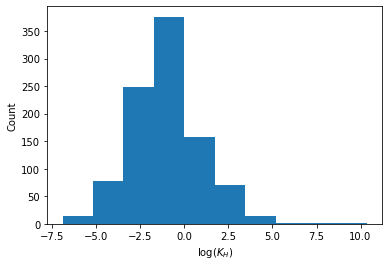
\includegraphics[width=4in]{data-dist.png} 
   \caption{The Distribution of $\log K_H$, where $K_H$ refers to the Henry's Law Constant.}
   \label{fig:dist}
\end{figure}


\section{Methods}
To model and predict chemical behavior, there are generally two schools of thought: use physiochemical descriptors to create a tabular representation of a molecule, or use the actual structure itself \cite{Ramsundar-et-al-2019}. Using just the structure itself is difficult, as unique representations of the molecule must be formed, and for a set of molecules, the model must be able to assess compounds with varying numbers of bonds and atoms. Historically, computational toxicologists have relied on algorithms that generate unique fingerprints for each molecule. These fingerprints can then be truncated so that each molecule has a representation with similar dimensions. However, graph neural networks have recently unencumbered computational toxicologists from requiring these fingerprints. To understand the efficacy of graph neural networks in the context of predicting Henry's Law, I created one model using physiochemical properties, one model using the fingerprint approach, and one model using graph neural networks.

To compare performance across models, I split the data into an 80\%/20\% train and test set, with hyperparameter tuning done using cross validation within the training set. Additionally, since the goal of each model is regression, I computed the $R^2$ value and the Mean Squared Error (MSE) on the training and test sets for each model.

\subsection{Using Physiochemical Properties}
Using the SMILES representation, the RDKit Feature Descriptors were queried to get a representation of the molecule containing 208 physiochemical properties. This list contained descriptors such as molecular weight and number of valence electrons, but also properties such as ring count, which means that this data contains some information about the structure beyond physiochemical properties. Since the goal of this section is to provide a baseline using simpler representations of the molecules, this data was kept.

Because this dataset is tabular, several models were initially attempted using SciKit Learn, since this package enables the quick training and evaluation of model performance \cite{scitkit-learn}. Models considered included a Random Forest Regressor, Ridge Regression, and K-Nearest Neighbors Regression. The highest $R^2$ value was achieved using the Random Forest Regressor with its default settings ($R^2=0.87$), whereas Ridge Regression and K-Nearest Neighbors Regression did not exceed $R^2= 0.81$ and $R^2=0.61$, respectively, under a variety of hyperparameter settings.

Random forest regression learns to model based off of generating an ensemble of decision trees, where each decision tree is given only a subset of the features. Each decision tree is generated by splitting the data based off of which feature split most decreases MSE. The random forest model then averages the predictions from each decision tree for its output. Given that the feature set is sparse for each compound, with only a subset of features being important within each subcategory, it makes sense that this model excels. Within the entire set of compounds, there are a few features that explain the variance, but within each subcategory, another set of features explain the variance within that subcategory. This is demonstrated in the supplemental material, in subsection 1, using principal components analysis, and it also demonstrates why dimensionality reduction attempts failed to improve model performance.

In a Random Forest model, several hyper parameters my be tuned to improve performance. The number of decision trees used can be increased to more permutations of the features and data, and overfitting can be prevented by constraining the learned trees to have a smaller max depth. Several values were considered to determine the optimal parameters by performing 4-fold cross validation on the training set. The optimal number of decision trees wound up being 200, with an optimal max depth of 10.


\begin{itemize}
	\item Using DeepChem, the features were extracted from RDKit.
	\item Features were visualized using Principal Component Analysis.
	\item A Random Forest model was chosen.
\end{itemize}

\subsection{Using Molecular Fingerprints}
% OMIT this section if you cannot fit...or just keep it short.
\begin{itemize}
	\item Transfer learning is beneficial because it uses information learned from previous work and applies it to new problems.
	\item This method of feature extraction was chosen because it is based on classical methods in computational toxicology, whereby a unique sequence representation of the molecule is based on the chemical structure (i.e.,, the Fingerprint method). Using Word2Vec, this sequence can be turned into a vector representation to be used in a regression model.
\end{itemize}

\subsection{Using a Graph Neural Network}

\begin{itemize}
	\item Graph Neural Networks have enjoyed considerable success using the structure of data for prediction.
	\item This final model was chosen because it achieves the goal of predicting Henry's law using minimal amount of data (just the structure of the molecule itself). 
	\item Graph representations were extracted using DeepChem's Graph Convolutional Featurizer, which is based on the WeaveNet model \cite{Kearnes2016}. 
	\item These representations along with their Henry's Law Constants were fed into a Graph Convolution Network (GCN), which is based on the model by \cite{Kipf2016}.
	\item Two other flavors of Graph Neural Networks were considered\: A graph attention network (GAT), as defined in \cite{Velickovic2017}, and a Message Passing Neural Network (MPNN), as defined in \cite{Gilmer2017}. However, initial performance on the validation set using the GCN exceeded performance on these alternative methods. Before hyperparameter tuning, the $R^2$ was 0.79 for the GCN, whereas the GAT and MPNN had $R^2$ values of 0.71 and 0.72, respectively.
	\item Talk about hyperparameter tuning.
\end{itemize}

\section{Results}
% Treat this as a discussion...
A summary of model performance is provided in Table~\ref{}

% Requires the booktabs if the memoir class is not being used
\begin{table}[htbp]
   \centering
   %\topcaption{Table captions are better up top} % requires the topcapt package
   \begin{tabular}{c c c c c} % Column formatting, @{} suppresses leading/trailing space
      \toprule

      Model    & Train $R^2$ & Test $R^2$ & Train MSE & Test MSE \\
      \midrule
      RF    & 0.97 & 0.87 & 0.13 & 0.50 \\
      GNN & 0 & 0 & 0 & 0 \\
      Opera & - & 0 & - & 0 \\
      \bottomrule
   \end{tabular}
   \caption{Remember, \emph{never} use vertical lines in tables.}
   \label{tab:booktabs}
\end{table}





\section{Discussion}

% ADDED 4/22/2022 -- not sure if this should be in the paper or not.
Previous research has achieved stellar performance predicting Henry's law. In \cite{English2021}, an $R^2$ value of 0.987 was reported on the test set. This model was a standard neural network.

\section{Conclusions}
I have created models using physical chemical properties, and models only using the structure, and these models perform very similarly. Given that my initial goal was to learn how to predict environmentally relevant chemical properties using only structure, my initial results suggest that this approach can be applied with success.

My next steps will be to determine whether alternative methods could improve performance. I suspect that my dataset size is preventing performance from increasing, so my focus will be on dimensionality reduction techniques and refined application of the embeddings provided by the Mol2Vec package. Previous research has demonstrated the efficacy of Variational Auto-Encoders applied to chemical footprints to enhance prediction of chemical toxicology \cite{RN106}. I believe a similar approach may be useful in this domain.

After applying this final approach, I will assimilate my approaches and compare them to the estimation approaches to further explore how my models are performing. I have created several models already, so further analysis is required to evaluate these models to understand the results so that my final report will contain more thorough analysis to better understand this problem space.

\section{IF I HAD MORE TIME}
I would do the following:
\begin{itemize}
	\item Work harder to compare the results from my model to the results reported in \cite{English2021}, as this model reports the best known results of the articles I consulted (REPORT THE RESULTS HERE). However, this model again restricted itself to a smaller set of compounds, and within compound categories, there was substantial variability. I want to evaluate my within group performance to determine results. The focus of future work needs to be on extrapolating outside of compound classes that are more well defined, as the harmful chemicals being discovered today lie outside of the categories defined in the article (CAN YOU \emph{SHOW} THIS?)
	\item Future work needs to additionally be on creating \emph{interpretable}, higher performant models, since those are the models used by practitioners in the field. I benchmarked my model against what practitioners reference (the EPA CompTox dashboard). I believe it was \cite{Mansouri2018} that said that these models need to be interpretable...now why is that?
\end{itemize}

\newpage
\section{Supplemental Material}

\subsection{Analysis of Principal Components}
To analyze how the data using physiochemical properties varies, Principal Component Analysis was used. When graphing the data into the first two principal components, for all subcategories, the first principal component explains only a small number of molecules, with most of the variance along principal component 2, as shown in Figure~\ref{fig:pc1}.

\begin{figure}[!h] %  figure placement: here, top, bottom, or page
   \centering
   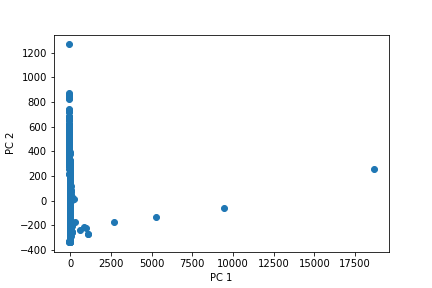
\includegraphics[width=4in]{PCA_all.png} 
   \caption{Principal Components for all of the data}
   \label{fig:pc1}
\end{figure}

However, if we look at the principal components within a specific subcategory, as shown in Figure~\ref{fig:pc2}, we see that the principal components look drastically different, with the molecules within the subcategory (labelled subcategory 40) demonstrating uniformity, and a potential third principal component explaining a large portion of the remaining variance.

\begin{figure}[!h] %  figure placement: here, top, bottom, or page
   \centering
   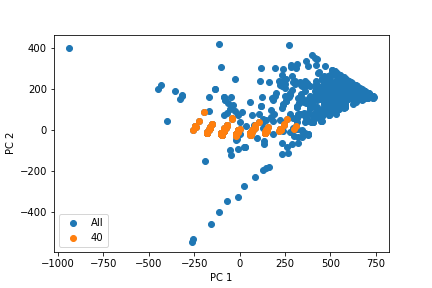
\includegraphics[width=4in]{PCA_subcat40.png} 
   \caption{Mapping data into the principal components for one subcategory}
   \label{fig:pc2}
\end{figure}

This suggests that the components that explains the variance in one subcategory does not explain the variance of the data as a whole. 

\bibliography{ds4cee-final-project}{}
\bibliographystyle{ieeetr}

\end{document}  